\chapter{Parallelization}

Here we describe how we can partition the algorithm to support parallelism.
A proof of concept for fully parallelized code can be seen in appendix A.

\section{Process}

The main process of the algorithm as described by dataflow diagram.\cite{Kahn74,Lee95}

\begin{figure}[H]
	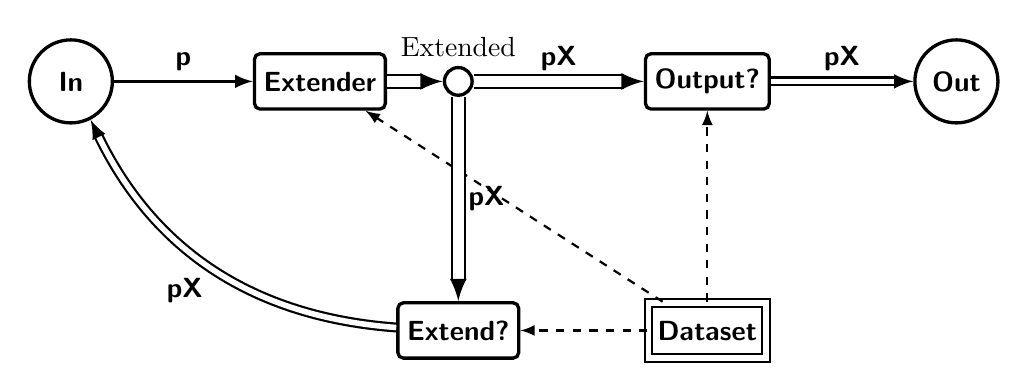
\begin{tikzpicture}[auto]
	\tikzstyle{pool} = [
		draw, very thick, fill=white, 
		circle,
		minimum height=3em, minimum width=3em, 
		node distance=9em, font={\sffamily\bfseries}];
	\tikzstyle{temppool} = [
		draw, very thick, fill=white, 
		circle,
		minimum height=1em, minimum width=1em, 
		node distance=5em, font={\sffamily\bfseries}];

	\tikzstyle{filter} = [
		draw, very thick, fill=white, 
		rectangle, rounded corners=0.2em,
		minimum height=2em, minimum width=4em,
		node distance=9em, font={\sffamily\bfseries}];
	\tikzstyle{extender} = [
		draw, very thick, fill=white, 
		rectangle, rounded corners=0.2em,
		minimum height=2em, minimum width=4em,
		node distance=9em, font={\sffamily\bfseries}];

	\tikzstyle{dataset} = [
		draw, thick, fill=white, 
		rectangle, double, double distance=2pt,
		minimum height=2em, minimum width=4em,
		node distance=9em, font={\sffamily\bfseries}];

	\tikzstyle{take} = [
		very thick, ->, >=latex,
		text centered, font={\sffamily\bfseries}];
	\tikzstyle{chan} = [
		thick, ->, >=latex, double, double distance=4pt,
		text centered, font={\sffamily\bfseries}];
	\tikzstyle{filtered} = [
		thick, ->, >=latex, double, double distance=2pt,
		text centered, font={\sffamily\bfseries}];
	\tikzstyle{needs} = [
		thick, ->, >=latex, dashed,
		text centered, font={\sffamily\bfseries}];

	\node[pool] (in) {In};
	\node[extender, right of=in] (ext) {Extender};
	\node[temppool, right of=ext, label=above:Extended] (exts) {};
	\node[filter, right of=exts] (outable) {Output?};
	\node[filter, below of=exts] (extable) {Extend?};
	\node[pool, right of=outable] (out) {Out};

	\node[dataset, right of=extable] (dataset) {Dataset};
	\draw[needs] (dataset) to (ext);
	\draw[needs] (dataset) to (outable);
	\draw[needs] (dataset) to (extable);

	\draw[take] 
		(in) to node{p} (ext);
	\draw[chan]
		(ext) to (exts);
	\draw[chan] 
		(exts) to node{pX} (outable);
	\draw[chan] 
		(exts) to node{pX} (extable);
	\draw[filtered, bend left] 
		(extable) to node{pX} (in);
	\draw[filtered]
		(outable) to node{pX} (out);
\end{tikzpicture}

\end{figure}

\todo{use proper syntax for dataflow diagrams}

Here we can see that the only dependence between query extending is the original dataset.

\section{Adding Nodes}

We can have multiple \emph{in} nodes if the \emph{extender} knows from where to fetch the \emph{querys}, which would require an additional scheduler.

This means that we can run several \emph{extenders} in parallel without effecting the overall process. Although we introduce a source for indeterminism.

\section{Extending}

Since much of the work is done in \emph{extender} we should also try to parallelize it as well:

\begin{algorithm}[H]
	\caption{Parallel Extender with Group optimization}
\begin{algorithmic}[1]
	\Require{Query $q$, function $next : \sym{I} \rightarrow [(\sym{I}, \sym{P})]$ }
	\Ensure{Set of querys that have been extended by one step}

	\Statef{ nexts \gets map(next, positions(q.matches)) }
	\Statef{ matches \gets groupBy(fst, nexts) }
	\Statef{ result \gets map(queryMaker(q), matches) }
	\Statef{ optimized \gets map( (x) \rightarrow (union(matches(x))), groups) }
	\Statef{ return union(result, optimized)}
\end{algorithmic}
\end{algorithm}

\todo[inline]{figure out how to make it readable}

\section{Dataset partitioning}

Since the dataset itself can be large it would be useful to divide it into parts. 

As we can see the extender only needs that sequences are intact, hence we can do the extension on partitioned dataset.

If we look at where we need synchronization points if we partition 
the dataset. Whole parts of extension still apply for parts of dataset.

The whole dataset is required only for filtering, since even one of the simplest operations ("counting matches in dataset") requires full knowledge of all matches over the dataset. But many such features can be calculated on sharded dataset with map-reduce.

\todo[inline]{example how to do counting}

There are also operations that require presence of all information or extended synchronization. One of the examples implemented in SPEXS is finding minimal p-value by splitting the data.

\todo[inline]{explain the optimal finding}

\section{Parallelized Process}

Applying these techniques we get a parallel dataflow:

\missingfigure{fully parallelized dataflow diagram}